\documentclass[tikz,border=2pt]{standalone}
\usepackage{amsmath,amssymb}
\usepackage{tikz}
\usetikzlibrary{matrix}

\begin{document}
% Independent X and Y: the joint pmf table is the outer product of the two marginals, every
% cell being P(X=x) P(Y=y).
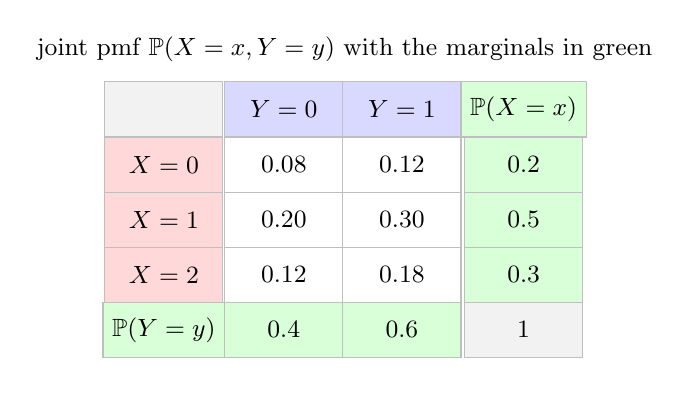
\begin{tikzpicture}[every node/.style={font=\small}]
	\matrix (T) [matrix of math nodes, nodes={minimum width=1.5cm, minimum height=7mm, anchor=center, draw=gray!50}, column sep=-\pgflinewidth, row sep=-\pgflinewidth] at (0,0) {
		|[fill=gray!10]| & |[fill=blue!15]| Y=0 & |[fill=blue!15]| Y=1 & |[fill=green!15]| \mathbb{P}(X=x) \\
		|[fill=red!15]| X=0 & 0.08 & 0.12 & |[fill=green!15]| 0.2 \\
		|[fill=red!15]| X=1 & 0.20 & 0.30 & |[fill=green!15]| 0.5 \\
		|[fill=red!15]| X=2 & 0.12 & 0.18 & |[fill=green!15]| 0.3 \\
		|[fill=green!15]| \mathbb{P}(Y=y) & |[fill=green!15]| 0.4 & |[fill=green!15]| 0.6 & |[fill=gray!10]| 1 \\
	};
	\node[anchor=south, font=\small] at (T.north) {joint pmf $\mathbb{P}(X=x,Y=y)$ with the marginals in green};
	
\end{tikzpicture}
\end{document}
